%%%%%%%%%%%%%%%%%%%%%%%%%%%%%%%%%%%%%%%%%
% Imperial Placement Report Template 
% LaTeX Template
% Version 1.0 (28/06/16)
% Version 1.1 (20/01/28) 
% Modified by Aufar Laksana into a lab report template
% For academic use only
%%%%%%%%%%%%%%%%%%%%%%%%%%%%%%%%%%%%%%%%%
%----------------------------------------------------------------------------------------
%	PACKAGES AND OTHER DOCUMENT CONFIGURATIONS
%----------------------------------------------------------------------------------------

\documentclass[12pt,a4paper]{report}
\usepackage[english]{babel}
\usepackage[utf8x]{inputenc}
\usepackage{amsmath}
\usepackage{amsfonts}
\usepackage{graphicx}
\usepackage{fancyhdr}
\usepackage[colorinlistoftodos]{todonotes}
\usepackage[toc,page]{appendix}
\usepackage{listings}
\usepackage[page]{totalcount}
\usepackage{color}
\usepackage{geometry}
\usepackage{caption}
\usepackage{subcaption}
\usepackage{float}
\usepackage[bottom]{footmisc}
\usepackage{diagbox}
\usepackage{gensymb}
\usepackage{mathpazo}

\usepackage{wrapfig}
\usepackage{lscape}
\usepackage{rotating}
\usepackage{epstopdf}


\usepackage{natbib} 



\definecolor{mygreen}{rgb}{0,0.6,0}
\definecolor{mygray}{rgb}{0.5,0.5,0.5}
\definecolor{mymauve}{rgb}{0.58,0,0.82}
\definecolor{mylilas}{RGB}{170,55,241}

\pagestyle{fancy}
\fancyhf{}
\lhead{Final Year Project}
\rhead{Interim Report}
\rfoot{\thepage\ / \totalpages}

% \geometry{headheight=15pt}
% \geometry{footskip=0.4in}
% \geometry{textheight=694pt}
% \geometry{textwidth=400pt}



\lstset{ %
  basicstyle=\small,
  backgroundcolor=\color{white},   % choose the background color; you must add \usepackage{color} or \usepackage{xcolor}; should come as last argument
  breaklines=true,                 % sets automatic line breaking
  captionpos=b,                    % sets the caption-position to bottom
  commentstyle=\color{mygreen}\ttfamily\small,    % comment style
  escapeinside={\%*}{*)},          % if you want to add LaTeX within your code
  extendedchars=true,              % lets you use non-ASCII characters; for 8-bits encodings only, does not work with UTF-8
  frame=shadowbox,	                   % adds a frame around the code
  rulesepcolor=\color{teal},
  keepspaces=true,                 % keeps spaces in text, useful for keeping indentation of code (possibly needs columns=flexible)
  keywordstyle=\color{blue},       % keyword style
  language=C,                 % the language of the code
  morekeywords={*,...},            % if you want to add more keywords to the set
  numbers=left,                    % where to put the line-numbers; possible values are (none, left, right)
  rulecolor=\color{black},         % if not set, the frame-color may be changed on line-breaks within not-black text (e.g. comments (green here))
  showspaces=false,                % show spaces everywhere adding particular underscores; it overrides 'showstringspaces'
  showstringspaces=false,          % underline spaces within strings only
  showtabs=false,                  % show tabs within strings adding particular underscores
  stringstyle=\color{mymauve},     % string literal style
  tabsize=2,	                   % sets default tabsize to 2 spaces
}
\lstdefinelanguage{Mymatlab}{
    language=Matlab,%
    %basicstyle=\color{red},
    basicstyle=\ttfamily\footnotesize,
    breaklines=true,%
    morekeywords={matlab2tikz},
    keywordstyle=\color{blue},%
    morekeywords=[2]{1}, keywordstyle=[2]{\color{black}},
    identifierstyle=\color{black},%
    stringstyle=\color{mylilas},
    commentstyle=\color{mygreen},%
    showstringspaces=false,%without this there will be a symbol in the places where there is a space
    numbers=left,%
    numberstyle={\tiny \color{black}},% size of the numbers
    numbersep=9pt, % this defines how far the numbers are from the text
    emph=[1]{for,end,break},emphstyle=[1]\color{red}, %some words to emphasise
    %emph=[2]{word1,word2}, emphstyle=[2]{style},    
}
\lstdefinelanguage{TI}{
  sensitive = true,
  keywords={MVC,MVK,MVKLH,LDDW,LDW,NOP,STW,ZERO,LDDW,MPYDP,ADDDP,SUB,B},
  otherkeywords={% Operators
    >, <, ==
  },
  keywords = [2]{_circ_FIR_DP,loop,lend},
  keywordstyle=\color{blue},
  keywordstyle=[2]\color{purple},% for example
  numbers=left,
  numberstyle=\scriptsize,
  stepnumber=1,
  numbersep=8pt,
  showstringspaces=false,
  breaklines=true,
  frame=shadowbox,	                   % adds a frame around the code
  rulesepcolor=\color{teal},
  comment=[l]{;},
  morecomment=[s]{/*}{*/},
  commentstyle=\color{mygreen}\ttfamily\small,
  stringstyle=\color{red}\ttfamily,
  morestring=[b]',
  morestring=[b]"
  }


\begin{document}

\begin{titlepage}


\newcommand{\HRule}{\rule{\linewidth}{0.5mm}} % Defines a new command for the horizontal lines, change thickness here
\setlength{\topmargin}{0in}
\center % Center everything on the page
 
\vspace*{-3cm}
 
\begin{minipage}{0.4\textwidth}
\begin{flushleft} \large
\hspace*{-0.5cm}
%\includegraphics[scale=0.14]{Imperial.png}\\
\end{flushleft}
\end{minipage}
~
\begin{minipage}{0.5\textwidth}
\begin{flushright} \large
\hspace*{2cm}
% \includegraphics[scale=0.4]{dsk6713.jpg}\\
\end{flushright}
\end{minipage}\\[1cm]
%----------------------------------------------------------------------------------------
%	HEADING SECTIONS
%----------------------------------------------------------------------------------------

\textsc{\LARGE Imperial College of Science, Technology and Medicine}\\[1.5cm] % Name of your university/college
\textsc{\Large Department of Electrical and Electronic Engineering}\\[0.8cm] % Major heading such as course name
\textsc{\Large  Final Year Project}\\[0.8cm] % Minor heading such as course title

%----------------------------------------------------------------------------------------
%	TITLE SECTION
%----------------------------------------------------------------------------------------

\addvspace{1.8em}

\HRule \\[0.2cm]
{ \huge \bfseries Interim Report:\\ Augmented Reality for Human Robotic Interaction }\\[0.2cm] % Title of your document
\HRule \\[1cm]
 
%----------------------------------------------------------------------------------------
%	AUTHOR SECTION
%----------------------------------------------------------------------------------------

\begin{flushleft}

\large \emph{Authors:} \\
Aufar \textsc{Laksana} \\
CID: 01093575\\

\addvspace{0.6em}

\large \emph{Project Supervisor:} \\
Dr. Yiannis Demiris\\

\addvspace{0.6em}

%\large \emph{Project Second Marker:} \\
%Dr. David Thomas\\

\addvspace{1.8em}

\end{flushleft}

% \begin{minipage}{1\textwidth}
% 	\begin{center}
% 		\frame{\includegraphics[scale=0.9]{declare.png}}\\
% 	\end{center}
% \end{minipage}\\[1cm]


\vspace*{3em}

%----------------------------------------------------------------------------------------
%	DATE SECTION
%----------------------------------------------------------------------------------------

{\large \today}\\[0.5cm] % Date, change the \today to a set date if you want to be precise


\vfill % Fill the rest of the page with whitespace
\end{titlepage}

\addvspace{6em}

\renewcommand{\abstractname}{\LARGE Abstract}

\tableofcontents
\newpage

\setlength{\parindent}{0pt}
\setlength{\parskip}{10pt}

\setlength{\belowcaptionskip}{-10pt}

\chapter{Introduction and Requirements}

\section{Introduction}
This report was written as part of the Final Year Project for the MEng. Electronic \& Information Engineering course. The project is supervised by Dr. Yiannis Demiris at the Imperial College London. The content of the report covers the research and progress of the project so far, between October 2018 until January 2019.

\section{Motivation}
A study on powered wheelchair users showed that there were approximately 3.6 million wheelchair users in the United States alone \citep{Kairy2014}. The study also showed that approximately 30\% of the users were operating powered wheelchairs (PWCs) or scooters, and that similar data had been reported in Europe. According to a report examining the recent trends amongst adults aged 65 and older in the United States, the number of elderly adults is projected to more than double from 46 million to over 98 million by 2060; due to increased life expectancy stemming from better healthcare and a reduction in mortality rate at older ages \citep{Mather2015}. As a result of the growing elderly population, it is likely that the number of powered mobility devices will continue to grow.

The study by \cite{Kairy2014} also highlights the problems faced by powered wheelchair users (PWUs). PWUs are often afraid of navigating in crowded areas, or are unable to operate their device safely, due to visual, motor and cognitive disabilities. In order to address these issues, the implementation of smart or intelligent wheelchairs has been proposed. These smart wheelchairs will help the users by providing services such as navigation assistance, allowing the user to carry out daily activities with more ease. An example of navigation assistance is collaborative control, \cite{Carlson2012} which utilizes a smart system that recognizes and assists the user when they require help, by manipulating the control signals of the powered wheelchair.

Within the Personal Robotics Lab at the Imperial College London, a lot of work has been done on enhancing the powered wheelchair user experience. One approach, \cite{Zolotas2018} involves the use of an augmented reality (AR) headset to help the user understand their wheelchair's behaviour. The AR headset renders helpful indicators, such as the trajectory of the wheelchair and highlighting potential obstacle collisions.

This project explores the idea implementing a smart system that would further benefit PWUs, by allowing them to navigate in crowded areas and recognizing locations that are frequently visited, such as at home or the shopping mall, and building a map of the location to allow better navigation assistance. An AR headset can also be utilized to display the internal state of the smart wheelchair, such as highlighting objects that determine the frequently visited location, or alerting the user to people moving towards the wheelchair and rendering a suggested path to avoid collision.

\section{Project Specification} \label{Project_Spec}
The aim of this project is to design and build a system that will allow powered wheelchair users to more easily conduct routine tasks, such as navigating around the house, or other frequently visited locations, such as the grocery store.

This project involves several hardware components, all of which are available within the Personal Robotics Lab. The hardware includes the following, as well as the sensors already mounted on the wheelchair:

\begin{itemize}
	\item Powered Wheelchair
	\item Microsoft Hololens
\end{itemize}

The system being developed is divided into two major parts, Robotic Behaviour and Augmented Reality Visualization.

\subsection{Robotic Behaviour}
The goal for this section of the project is to design and develop algorithms that will allow for assistive navigation on the powered wheelchair. The system will utilize sensors mounted on the wheelchair to build up a map of the surroundings. Objects in the surrounding area will be detected and marked as potential collisions, depending on the trajectory of the wheelchair. An extension is the ability to detect moving objects, such as people, calculating the trajectory of the object and deciding if a collision is imminent.

A major hardware component of this project is the Microsoft Hololens, a mixed reality headset that can be worn by the powered wheelchair user. The Hololens posses the ability to track the eye movements of the user with an eye-tracker addon. An interesting concept that can be explored is the ability to control the powered wheelchair using the eye-tracker, removing the need for a joystick, allowing users who lack the motor skills to operate the wheelchair. This feature can also be used to check if the user has noticed an object that may cause a collision. Should the user not see the object, the system will first highlight the object, before taking over from the user 

\subsection{Augmented Reality Visualization}
Using the Hololens, the goal of this section is to communicate to the user the internal state of the system controlling the powered wheelchair. Using augmented reality, visualizations will be rendered on the Hololens, allowing the user to understand the trajectory of the wheelchair, what potential collisions may occur. The system will also be able to take over control of the wheelchair, as such, it would be beneficial if a warning was displayed to the user right before the system takes over.

Other visualizations include highlighting moving objects and tracking them as they move across the field of vision of the user. Should the user not notice a moving object that may cause a collision, the Hololens will flash a warning and highlight the object in order to attract the attention of the user, allowing them to make adjustments themselves.

\newpage

\chapter{Literature Review}

\section{Object Detection}
In this project, the main purpose of object detection algorithms will be to identify objects of the class 'Human' in the surrounding area of the wheelchair. In order to tackle the problem of users being unwilling to navigate in crowded areas, a system must be implemented to help track and navigate around humans.

One of the modern approaches to detecting humans in an image from a camera is to use Deep Convolutional Neural Networks. Human detection,as stated by \cite{Vidanapathirana}, is a special case of Object Detection and Object Localization. The system would ideally be able to pinpoint the location of the human object relative to the wheelchair, in order to be able to calculate the trajectory of the person.

However, the use cases of object detection is not only limited to detecting humans. There has been research conducted into the use of object detection for recognizing the scene around a robot, ie. the system is able to identify the robot is now in a hallway \citep{Quattoni2009, Espinace2010}.

\subsection{Human Detection}
The main challenges with detecting humans in an image is the large variations in the appearance. A frontal view of a person may be recognized by the algorithm, but a side view may cause problems due to the algorithm not recognizing key features from a different angle \citep{Dalal2004}.

\paragraph{SIFT} A solution to this problem is outlined by \cite{Lowe2004}, in an approach named the Scale Invariant Feature Transform (SIFT), which transforms image data into co-ordinates which are scale invariant relative to local features. This method allows for a large number of features to be extracted from an image. The feature are also distinct, allowing for a single feature to be correctly matched with a low uncertainty against a database of existing features.

A large quantity of features is required for object detection, due to the often cluttered nature of the image. In order to detect a small object in the background, at least 3 features must be correctly matched for reliable identification. 

In order to perform object detection, SIFT features are first extracted from the training set of available images. A new image, in our case, a human torso/body, will be recognized by individually comparing the features in the test image with the features in the training set, in a Nearest Neighbours approach utilizing Euclidean distance. However, a drawback of using SIFT is the high computational cost of comparing the features \citep{Wang2011}.

\paragraph{YOLO}
You Only Look Once (YOLO) is a state of the art object detection system relying on a single neural network to predict bounding boxes around the objects \citep{Redmon2015}. The main advantage of YOLO is that it is extremely fast, as the name, the algorithm only looks once at an image to predict what objects are present.

\begin{figure}[h!]
	\begin{center}
		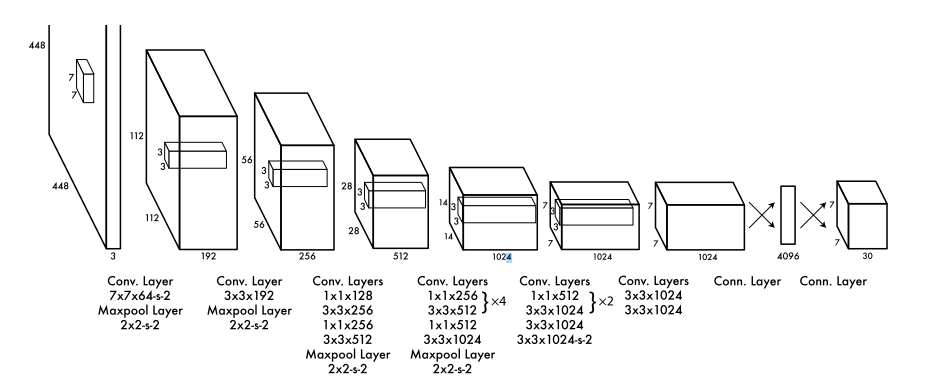
\includegraphics[scale=0.4]{Images/Literature/YOLO_Architecture.png}
		\caption{The YOLO architecture \citep{Redmon2015}}
	\end{center}
\end{figure}

The Convolutional Neural Network (CNN) in the YOLO system takes in an image and resizes it to 448x488 pixels. The image is then passed through the CNN layers and is output as a 7x7x30 tensor, containing the co-ordinates of the bounding boxes and the probability distributions over all the classes the network is trained on. 

The YOLO algorithm has been used to recognize human actions by \cite{Shinde2018}, using the LIRIS Human Activities dataset, which contain human actions such as shaking hands and entering rooms. It was found in the study that only a few frames of a streamed video is required for the YOLO algorithm to recognize the human actions.

\begin{figure}[h!]
	\begin{center}
		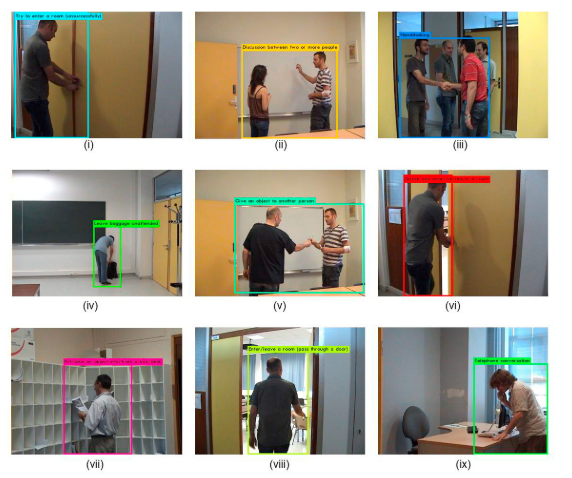
\includegraphics[scale=0.4]{Images/Literature/YOLO_Action_Recognition.png}
		\caption{The YOLO algorithm recognizing human actions \citep{Shinde2018}}
	\end{center}
\end{figure}

An extension of this work for the purposes of this project would be to detect humans walking towards the camera mounted on the wheelchair, in order to help with navigating through crowded areas.


\section{Simultaneous Localization And Mapping (SLAM)}
The term mapping refers to a system that will create a map of the surrounding areas, by detecting objects such as walls and other obstacles. In order to help users navigate, the system must analyse the surroundings for potential dangers. As such, it is important to build up a thorough and complete map.

A fundamental method for robot navigation is the Simultaneous Localization And Mapping (SLAM) method. The process allows the system to predict the trajectory of the robot and the location of all objects on-line, without the need of an \textit{a priori} knowledge of the robots location \citep{Bailey2006a}. The method estimates the pose of the robot relative to landmarks which are detected. The popularity of SLAM increased with the emergence of indoor applications of robotic devices. For this project, it is expected that the user will be mostly navigating around the house or indoors, which rules out the use of GPS to bound the localization errors \citep{Cadena2016}.

\subsection{Existing Work}
A review of SLAM techniques can be found in \cite{Cadena2016}, which also outlines the standard formulation of the SLAM problem as that of a Maximum a posteriori (MAP) estimation. The formulation relies on Bayes theorem, and using the prior knowledge of the robots pose to maximize the likelihood to estimate the current position of the robot. The variables required to estimate the position are the robot poses, the position of landmarks and the calibration parameters of the sensors.

In order to build an accurate map of the surroundings, the calibration of the sensors providing the measurements is a crucial step. The choice of sensors also matter, as the type of data returned by the sensor may affect the computational complexity of the SLAM algorithm. As such, it is common to have a module in the system that deals with the extraction of relevant features from the sensor data.

A fairly common assumption in SLAM approaches is that the world is static and remains unchanged as the robot moves. This becomes an issue with the goal of this project, which hopes to achieve the ability to detect human objects walking around the wheelchair. This issue will be addressed in a later section.

\subsection{Visual SLAM}
Visual SLAM (vSLAM) is an implementation of SLAM that relies on visual inputs only. As stated in \cite{Taketomi2017}, vSLAM is suitable for AR due to the low computational algorithms that can be implemented on the limited resources of an AR headset. The technique of vSlam is mainly composed of three modules:

\paragraph{Initialization}
In the initialization stage, camera pose estimation is conducted, to transform objects in a 2D image from the camera into a 3D co-ordinate system that the robot understands. This process determines the position and orientation of the camera relative to the object. A part of the environment is reconstructed as part of the initial map using the global co-ordinate system of the robot.

\paragraph{Tracking}
Here, the reconstructed map is used to estimate the pose of the camera with respect to the map. Feature mapping or feature tracking is conducted on the images in order to get a 2D-3D correspondence between the image and the map. The camera pose can then be calculated from the correspondences by solving the Perspective-n-Point problem \citep{Nister2004}. This allows the system to identify where on the map the robot currently is.

\paragraph{Mapping}
When the robot passes through an environment that has previously not been mapped, the 3D structure of the surroundings is calculated from the camera images. The structures are then added to the existing map of the environment.

\section{Scene Recognition} \label{section:Scene_Recognition}
Wheelchair users spend a substantial part of their time at home. An active area of research called assistive domotics \citep{Rosslin2010}, involves developing assistive technology and home automation systems that allow users to interact with common household objects from a seated position in the wheelchair.

The ability for a smart wheelchair to recognize a room in the house would greatly improve the user experience. A map of the surroundings that was previously built of that room can now be loaded when the wheelchair enters the room again, greatly reducing the amount of computational overhead in rebuilding the entire map. The stored maps may contain useful information such as the positions of doorways or other objects of interest that the users can interact with.

\cite{Quattoni2009} proposed a scene recognition model that is specifically built for recognizing indoor scenes, by using image prototypes to learn a distance function to map indoor scenes to their correct labels. Scenes containing similar objects tend to have the same labels, and it was found that some objects are more important than others in determining a scenes identity. For instance, a library will contain many bookshelves, whereas a kitchen is unlikely to. A similar method is proposed by \cite{Espinace2010}, which relies on object detection to correctly classify scenes. The intuition is that objects can be detected in real time, and using contextual relations, it is possible to associate objects with scenes.

\section{Head Mounted Display and Control}

\subsection{Microsoft Hololens}
The Microsoft Hololens is an untethered holographic computer, allowing for the display of 3D holograms pinned to real world objects. The Hololens is equipped with an array of sensors, making it an ideal choice of hardware for this project.

\begin{figure}[h!]
	\begin{center}
		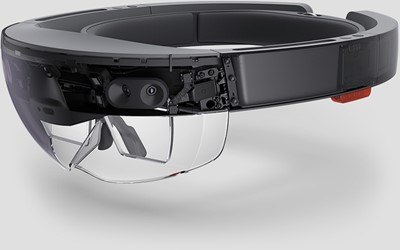
\includegraphics[scale=0.4]{Images/Literature/hololens.jpg}
		\caption{The Microsoft Hololens hardware \citep{Zeller}}
	\end{center}
\end{figure}

\paragraph{Hardware Specifications}
The Microsoft Hololens contains the following sensors:

\begin{itemize}
	\item 1 Intertial Measurement Unit (IMU)
	\item 4 Environment understanding cameras
	\item 1 Depth Camera
	\item 1 2MP Photo/HD video camera
	\item Mixed reality capture
	\item 4 Microphones
	\item 1 Ambient Light Sensor
\end{itemize}

A full technical specifications for the hardware is available from \cite{Microsoft2015}.

\paragraph{Development}
Mixed Reality applications are developed using the Universal Windows Platform. A computer running Windows 10 will be required to develop applications, since programs such as Unity and Microsoft Visual Studio will need to be installed.

\paragraph{Gaze}
The concept of Gaze is that of a form of targeting in mixed reality applications \citep{Microsoft}. It lets the system to know where the user is looking in the world, and from there, allows the system to discern their intent. Users tend to look at the object or location that they will interact with.

Using the Hololens, a mixed reality application can determine whether a user is currently not looking at an object, allowing the application to give a visual/audio cue to the user to look at the object. This can be used in this project to alert the user to a potential collision with a  person that is approaching the wheelchair if the user has not spotted the person already.


\paragraph{No Eye Tracker}
The Hololens can keep track of its location and rotation relative to the environment, but is unable to capture eye gaze data. This is because there are no internally facing cameras. The user can interact with virtual objects by using a virtual cursor, controlled by changing their physical position and head rotations. Applications can be developed to estimate where the user is looking while wearing the device. 

Relying on head gaze to estimate the point that a user is looking at is limited in its accuracy, since the users eyes can move away from the centre of the Hololens, so the user is actually looking at something else. In the research by \cite{VanderMeulen2017}, an extra eye-tracker from Pupil Labs was attached to the Hololens. It was found that the addition of the eye-tracker greatly increased the accuracy in gaze location calculations. For virtual targets, the eye-tracker had a minimal effect on the estimation, and can be estimated by head rotation alone.

\subsection{Augmented Reality Visualization}
The Microsoft Hololens is able to blend real world and virtual content into environments where digital and physical objects can co-exist and interact. The term 'Mixed Reality' was first introduced by \cite{Milgram1994}, and refers to the blending of the physical and virtual worlds.

The Hololens allows the developer to create 'Holograms', which are objects of light and sound that are displayed by the headset. Users are able to interact with the holograms through voice, gaze and gestures. Enhanced environment apps are applications that facilitate the placement of digital information on the user's current environment \citep{Microsofta}. An example of an enhanced environment application is placing markers in augmented reality on objects that the user can interact with in both the physical and digital worlds. 


\subsection{Gaze/Eye-Tracking Control}
The idea of gaze based control has already been explored in the Personal Robotics Lab \citep{Chacon-Quesada}, by also using the Microsoft Hololens as an AR head-mounted display. It was shown that the user could control the smart wheelchair using the AR user interface, allowing them to navigate through doors and approach people.

\begin{figure}[h!]
	\begin{center}
		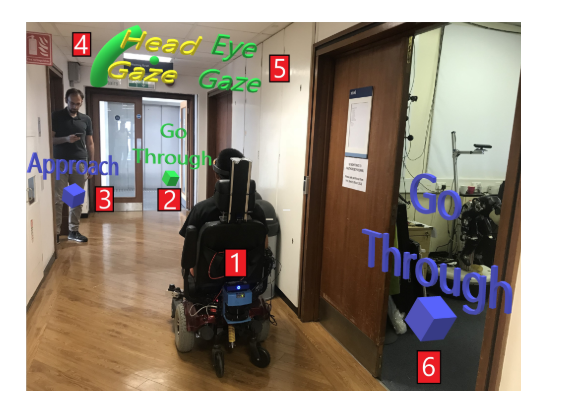
\includegraphics[scale=0.4]{Images/Literature/AR_Interface.png}
		\caption{The AR User Interface demonstrated by  \cite{Chacon-Quesada}}
		\label{fig:Chacon_AR}
		
	\end{center}
	
\end{figure}

The implemented system is aware of both humans and other objects in the surroundings, and allowing the user to select various options to interact with the objects, as seen in Figure \ref{fig:Chacon_AR}.

%\newpage

\cite{H.Montenegro-Couto2018} uses a concept whereby they use an eye-tracker to control the wheelchair motors via gaze rather than a joystick. The options to control the wheelchair are displayed on a screen, and the eye-tracker calculates the 2D co-ordinates of where the person is looking at on the screen. Various options are listed such as the ability to manoeuvre the wheelchair, as well as interact with nearby objects.

\begin{figure}[h!]
	\begin{center}
		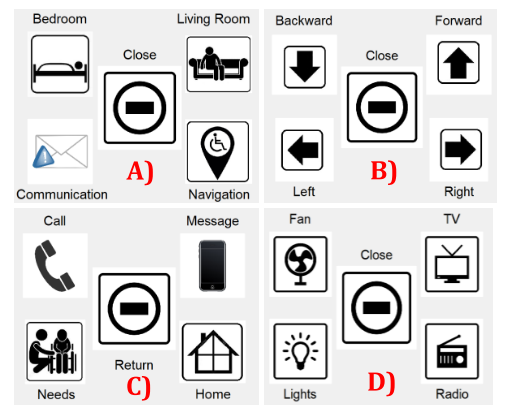
\includegraphics[scale=0.4]{Images/Literature/Eye_Tracker_Control.png}
		\caption{The screen displayed to users in \cite{H.Montenegro-Couto2018}}
	\end{center}
\end{figure}

\newpage

\section{Competing Products}
One of the main issues with gaze/eye based control is that of the 'Midas touch' problem, where every gaze does not equal a goal. The user may look at an object for a split second, but may not actually want to move towards that object. To counteract this problem, \cite{Wastlund2010} developed a system which displays on-screen buttons that control the wheelchairs movements. The system also stopped the wheelchair when the device approaches an object.

\begin{figure}[h!]
	\begin{center}
		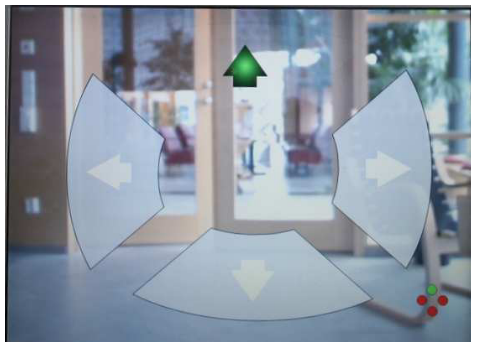
\includegraphics[scale=0.4]{Images/Literature/Wastlund_AR_Screen.png}
		\caption{The on-screen buttons displayed to users \citep{Wastlund2010}}
	\end{center}
\end{figure}

A similar idea was proposed by \cite{Arai2011}, whereby an eye-tracker would detect the position of the pupil and translate it onto an invisible control panel similar to that of \cite{Wastlund2010}. To avoid the Midas touch problem, a sustained gaze at one of the controls was required before the wheelchair would move.

\cite{Raymond2018} proposes a system which utilizes a depth camera in conjunction with an eye tracker. The system identifies between eye movements aimed at the floor as a gaze target and other non-navigational eye movements. This approach is different as it does not rely on an artificial user interface to control the wheelchair as proposed by \cite{Arai2011, Wastlund2010}.


\newpage
\chapter{Implementation Plan}
This section of the report goes over the overall project goals, as well as the steps that will need to be taken in order to achieve the goals within the given time frame.

\section{Overall Project Goals}
As mentioned in Section \ref{Project_Spec}, the goal of this project is to develop an intelligent powered wheelchair capable of recognizing objects and humans in its vicinity. By building a map of its surroundings, and through object detection, useful prompts can be displayed to the user. The ability to detect people will greatly decrease the possibility of a collision when navigating through more crowded spaces, and can be achieved by displaying alerts on the head-mounted AR device or through the system taking over control of the wheelchair to avoid the object.

Furthermore, the Microsoft Hololens forms a key part of the overall system design. By making use of the sensors available on the headset, such as the depth camera, as well as the Gaze method to estimate where the user is looking, another goal for this project is to implement a wheelchair control system that solely relies on head pose, rotation and gaze, removing the need for a joystick and allowing users who are paralysed to more easily control their powered wheelchair.

\section{Hardware Analysis}
Before any algorithms can be developed, it is important to understand the hardware available. For instance, camera resolution will affect the image quality, which may become an issue for object detection. As such, a proper analysis of any cameras, sensors and other pieces of hardware should be conducted.

\subsection{Powered Wheelchair}
The Personal Robotics Lab have built the Assistive Robotic Transport for Adults (ARTA), a smart powered wheelchair, which has been used for several other research projects \citep{Chacon-Quesada, Zolotas2018}. From the reports, it can be seen that ARTA already has some built-in obstacle avoidance and shared control methodologies.In addition, it is also equipped with laser range finders, which can return depth information. \cite{Chacon-Quesada} also utilizes the Hololens camera to capture images of the surroundings, but the main bulk of the image processing is done on a remote computer, which communicates with the head mounted display (HMD).

Further investigation into the sensors and other hardware on the wheelchair will need to be conducted, by asking members of the Personal Robotics Lab who have worked with the wheelchair. Official documentation for the wheelchair is sparse, and it would be less time consuming to ask people directly. Additionally, more sensors can be mounted on ARTA, should the need arise.

\subsection{Microsoft Hololens}
The Microsoft Hololens is a key component of the project, as it will be used to both obtain images and display AR visual cues by rendering holograms. The official documentation \citep{Microsofta} is available online, along with many tutorials on websites such as Youtube and Stackoverflow.

\subsubsection{Pupil Labs Eye-Tracker}
The Personal Robotics Lab also has access to an add-on for the Hololens, an eye-tracker developed by Pupil Labs. The cameras on the add on run at 120hz and low latency eye tracking software is available from the company, allowing for applications that require fast interaction \citep{PupilLabs}.

\subsubsection{Development}
Developing applications for the Hololens requires a computer running Windows 10, and installations of Microsoft Visual Studio, Unity and several other programs \citep{Microsofta}.

\subsection{Hardware Access and Additional Hardware}
As ARTA and the Hololens can not leave the Personal Robotics Lab, time slots for development time will need to be arranged with the other members of the lab. Furthermore, after analysing the sensors available on the wheelchair, more sensors may need to be requested. At the time of writing, a Xbox Kinect Camera is being considered as another camera that may be mounted on ARTA.


\section{Augmented Reality Wheelchair Control} \label{section:ARWC}
Utilizing the Microsoft Hololens and the Pupil Labs eye-tracker add-on, the goal of this part of the project is for the user to have the ability to stare at a location in front of the wheelchair, and the system will recognize the intent to move towards a goal. This intent is then converted to wheelchair control signals and the user will be able to navigate the powered wheelchair without the use of a joystick.

\subsection{Cross Platform Interface}
The wheelchair control relies on the Robotic Operating System (ROS), which runs on a standard Linux distribution such as Ubuntu 16.04. On the other hand, the Hololens runs on the Universal Windows Platform. As such, an interface between the two operating systems is needed. Members of the Personal Robotics Lab have already developed these interfaces for their previous projects.

\subsection{Eye-Gaze Estimation}
To allow the user to fixate their gaze on a specific point and navigate the wheelchair towards that point, an eye-gaze estimation system will need to be implemented. Using the eye-tracker and depth camera on the Hololens, and approach similar to the one used by \cite{Raymond2018} will be developed. It has been noted that head-gaze can be used to determine a goal destination, but as shown through the research of \cite{VanderMeulen2017}, there is a significant increase in the accuracy when used in conjunction with an eye-tracker, and it will also greatly reduce the Midas touch problem.

\section{Human Detection System} \label{section:HDS}
Previous research by \cite{Chacon-Quesada} utilizes the Detectron object detection method \citep{Detectron2018} and conducts the processing on a remote computer. For this project, the goal of the human detection would be to detect the human in the image, and using depth cameras or laser range finders, determine if the person is moving closer towards the wheelchair and if a collision is imminent.

A personal interest of mine is to work more with Deep Learning and Neural Networks in order to gain a better, practical understanding of the concept. As such, for this project, I would like to work with the YOLO object detection method to be able to recognize humans and track them across frames \citep{Shinde2018, Redmon2015}.

\subsection{Testing Pre-Trained Models}
There are already pre-trained YOLO networks capable of recognizing people. However, these need to be tested with the Hololens camera to see if the images produced by the Hololens will allow the networks to recognize people.

\subsection{Estimating Moving Human Trajectories}
In order for the wheelchair to be aware of potential collisions with humans, the people in the vicinity must be detected and considered as a landmark by the Visual SLAM system. A system utilizing vSlam and a Moving Object Detector similar to the work done by \cite{Wang2011} will be employed to locate the positions of people in the surroundings, and estimate their trajectories.


\section{Obstacle Avoidance System} \label{section:OAS}
The goal of the obstacle avoidance system is for the wheelchair to be intelligent in detecting obstacles in the surroundings. The system will encompass the Human Detection System mentioned in Section \ref{section:HDS} as well as using range finders and mapping techniques to prevent the user from colliding with walls and other obstacles.

\subsection{Utilizing Existing Work}
Previous work by \cite{Zolotas2018} uses various software and hardware components atop the Robotic Operating System, which estimate the trajectory of the wheelchair and render holograms on the HMD showing the current path, as well as a suggested path should the current trajectory result in a collision.

An extension of this would be for the system to realize when to take over from the user should they not respond to the visual warnings. The system will then manoeuvre the wheelchair into a trajectory it deems safe that will avoid the oncoming object.

\subsection{Hologram Warnings}
Utilizing the display on the Microsoft Hololens, once a human or object is detected, it will be tracked as it moves across the users field of view. However, users may not always spot the oncoming object, due to being distracted or looking elsewhere.

The Hololens and the Pupil Labs eye-tracker allow for a system to be developed which will know when the user has not spotted the oncoming object. When the system realizes this, a warning hologram will be rendered on the HMD, highlighting the oncoming object and alerting the user with a sound from the direction the object is coming from.

\section{Project Timeline}
The project timeline is listed in the Appendix Figures \ref{app:fig:timeline1} and \ref{app:fig:timeline2}. The Gantt chart displays the project outline, and what tasks are dependant upon each other.

\section{Fallback}
Should time constraints become an issue, the part of the project that can be reduced is the Obstacle Avoidance System outlined in Section \ref{section:OAS}. It may become too burdensome to implement a system that will take over control from the user and work reliably. As such, just displaying the warning to the user in the form of a hologram and forcing the wheelchair to stop if they do not pay attention to the warning will be a suitable reduction.

This will leave more time for testing of the Human Detection System ( Section \ref{section:HDS}) and the Augmented Reality Wheelchair control (Section \ref{section:ARWC}), which are considered as core components of this project, and will be demoed during the presentation.

\section{Extensions}
The following section outlines the possible extensions to the project, should time allow. The technical implementation details have not been fully researched, but a basis has been formed from the literature review.

\subsection{Scene Recognition}
As mentioned in Section \ref{section:Scene_Recognition}, Scene Recognition can be of used to aid powered wheelchair users conduct routine tasks. For instance, by recognizing the device has returned to an area marked as the user's home, it may be a good idea to turn off the human detection system, since it is unlikely that the user will encounter many people. This would reduce in the amount of computation going on in the background. Another use may be to load stored maps of an area that has been previously explored, such as a map of the house, and only unexplored or changed areas would be updated of the map.

As explored by \cite{Quattoni2009}, as well as \cite{Espinace2010}, object detection algorithms can be used to recognize scenes. By training the YOLO object detector to recognize objects other than humans, we may be able to map a relationship between objects and scenes.

This would involve training another convolutional neural network to recognize objects in an image from the Hololens, and associating that object with a label. An example of this would be recognizing pots and pans and labelling the scene as a kitchen. As such, an indoor scene dataset would be required to train the network, which would have to be gathered manually and labelled. An alternative would be to make use of indoor scene datasets previously used by \cite{Quattoni2009}.

\section{Overall System Architecture}
The high level overview of the project is displayed in the Appendix, Figure \ref{app:fig:System_Architecture}. An onboard computer running Linux will do most of the processing, such as the gaze-estimation and human detection. The Hololens will provide the Linux system with gaze and eye-tracker data, as well as the images for the YOLO human detector.

The individual units will communicate with the wheelchair control unit running on the Robotic Operating System. Stop signals are sent to the control unit when the human detector estimates that a collision is about to happen. The Eye-Gaze Estimation unit will send driving instructions to reach a point the user is looking at. 

\newpage
\chapter{Evaluation Plan}

\section{Human Detection Test}

\section{Eye-Gaze Control Test}

\section{Full System Test}


\newpage
\chapter{Ethical, Legal \& Safety Plan}

\newpage
\bibliographystyle{agsm}
\bibliography{FinalYearProject}

\newpage

\appendix
\pagestyle{fancy}
\fancyhf{}
\lhead{Final Year Project: Appendix}
\rhead{Interim Report}



\appendixpage

\begin{figure}[ht]
	\centering
	\begin{turn}{-90}
			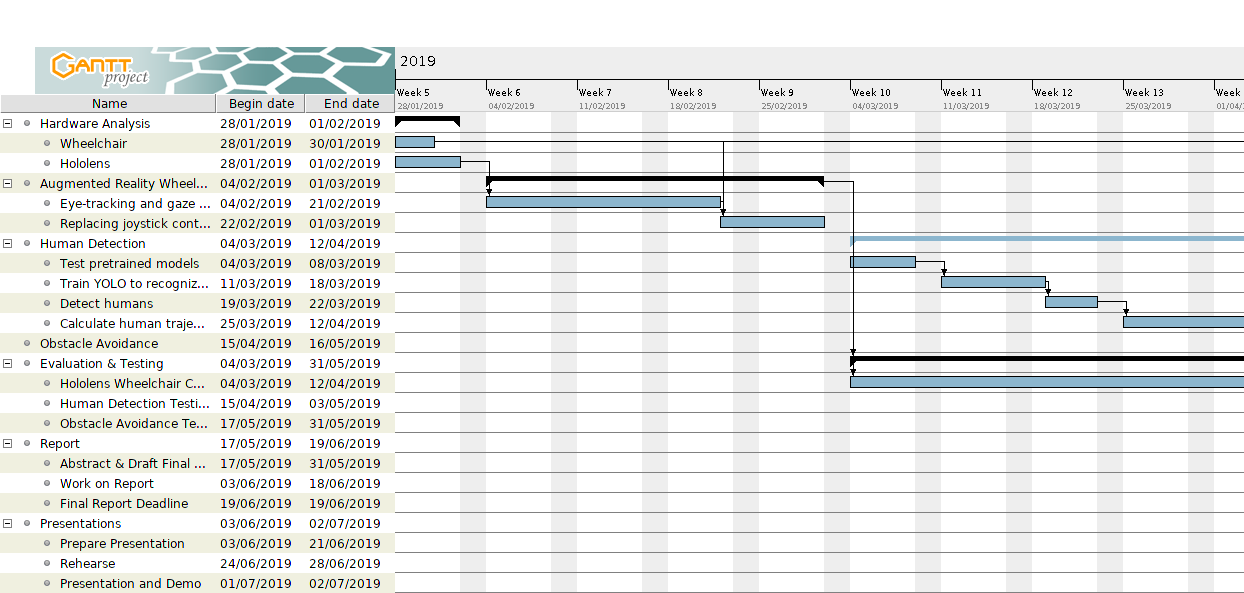
\includegraphics[scale=0.5]{Images/Implementation/Timeline_Split-0.png}
	\end{turn}
	\caption{Project Timeline (Part 1)}
	\label{app:fig:timeline1}
\end{figure}

\begin{figure}[ht]
	\centering
	\begin{turn}{-90}
		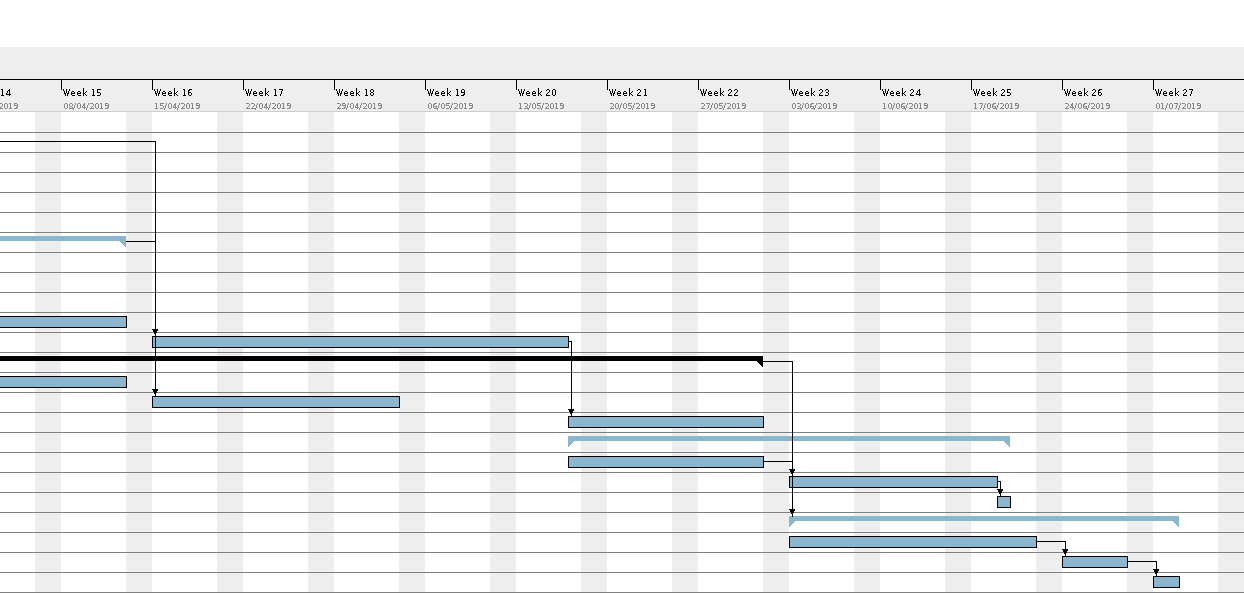
\includegraphics[scale=0.5]{Images/Implementation/Timeline_Split-1.png}
	\end{turn}
	\caption{Project Timeline (Part 2)}
	\label{app:fig:timeline2}
\end{figure}

\newpage

\begin{figure}[h]
	\begin{center}
		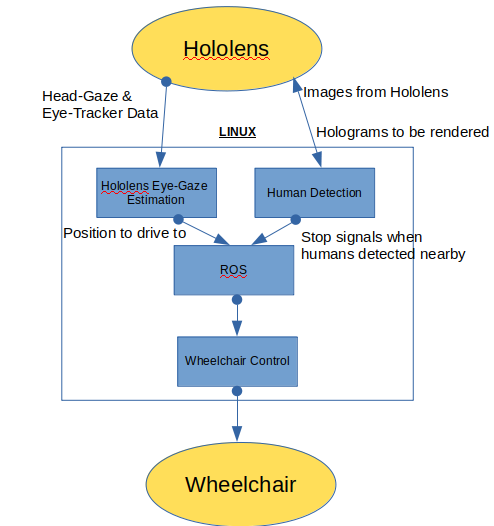
\includegraphics[scale=0.9]{Images/Implementation/System_Design.png}
		\caption{Overall System Architecture}
		\label{app:fig:System_Architecture}
	\end{center}
\end{figure}



\end{document}